\documentclass[12pt,a4paper]{report}
\usepackage{iftex}
\ifPDFTeX
  \usepackage[utf8]{inputenc}
  \usepackage[T5]{fontenc}
  \usepackage[vietnamese]{babel}
\else
  \usepackage{fontspec}
  \usepackage{polyglossia}
  \setdefaultlanguage{vietnamese}
  \setmainfont{Times New Roman}
\fi
\usepackage{geometry}
\usepackage{setspace}
\usepackage{graphicx}
\usepackage{float}
\usepackage{booktabs}
\usepackage{longtable}
\usepackage{array}
\usepackage{caption}
\usepackage{hyperref}
\usepackage{amsmath}
\usepackage{enumitem}
\usepackage{titlesec}
\usepackage[numbers,sort&compress]{natbib}

\geometry{left=3cm,right=2.5cm,top=2.5cm,bottom=2.5cm}
\setstretch{1.25}
\hypersetup{colorlinks=true,linkcolor=black,citecolor=black,urlcolor=blue}
\setlength{\parskip}{0.4em}
\setlength{\parindent}{1.2em}

\titleformat{\chapter}[display]
  {\normalfont\bfseries\Large}
  {CHƯƠNG \thechapter}
  {0.5em}
  {\LARGE}

\begin{document}

% Cover
\begin{titlepage}
    \centering
    {\large TRƯỜNG ĐẠI HỌC SÀI GÒN\par}
    {\large KHOA CÔNG NGHỆ THÔNG TIN\par}
    \vspace{2.0cm}
    {\Large\bfseries BÁO CÁO TIỂU LUẬN\\MÔN PHÂN TÍCH DỮ LIỆU\par}
    \vspace{1.5cm}
    {\Large\bfseries ĐỀ TÀI\par}
    \vspace{0.5cm}
    {\LARGE\bfseries RÚT TRÍCH DỮ LIỆU VÀ TIỀN XỬ LÝ\\DỮ LIỆU PIMA INDIANS DIABETES\par}
    \vspace{1.5cm}
    \begin{flushleft}
        \textbf{Giảng viên hướng dẫn:} ........................................\\
        \textbf{Nhóm thực hiện:} Nhom01\_SGU26\_ML\\
        \textbf{Học phần:} Học phần thay thế khóa luận
    \end{flushleft}
    \vfill
    {TP. Hồ Chí Minh, 2026\par}
\end{titlepage}

% Assignment
\chapter*{Phân công thành viên}
\addcontentsline{toc}{chapter}{Phân công thành viên}
\begin{longtable}{>{\raggedright\arraybackslash}p{3cm} >{\raggedright\arraybackslash}p{7.5cm} >{\centering\arraybackslash}p{2cm}}
\toprule
\textbf{Thành viên} & \textbf{Nhiệm vụ chính} & \textbf{Tỷ lệ}\\
\midrule
Chibang & Tổng hợp notebook, xây dựng pipeline tiền xử lý, tổng hợp báo cáo & 25\%\\
Duybao & Hỗ trợ kiểm tra notebook, đối chiếu kết quả và markdown diễn giải & 25\%\\
Tranhuyvu & Phân tích sâu cho nhóm biến BMI/Insulin, góp ý trực quan hóa & 25\%\\
Truongphat & Phân tích sâu cho nhóm biến Age/DPF, góp ý diễn giải kết quả & 25\%\\
\bottomrule
\end{longtable}

% Instructor comments
\chapter*{Nhận xét của giảng viên}
\addcontentsline{toc}{chapter}{Nhận xét của giảng viên}
\vspace{6cm}
\noindent\hrulefill\\[1.2cm]
\noindent\hrulefill\\[1.2cm]
\noindent\hrulefill

% Intro and thanks
\chapter*{Lời mở đầu}
\addcontentsline{toc}{chapter}{Lời mở đầu}
Báo cáo này trình bày kết quả thực hiện bài tập Lab 03 với dữ liệu Pima Indians Diabetes.
Nhóm tập trung vào hai mục tiêu: (1) xây dựng quy trình rút trích và tiền xử lý dữ liệu có thể tái lập;
(2) đánh giá các chiến lược tiền xử lý dưới góc nhìn mô hình học máy baseline.

\chapter*{Lời cảm ơn}
\addcontentsline{toc}{chapter}{Lời cảm ơn}
Nhóm xin chân thành cảm ơn giảng viên hướng dẫn đã cung cấp yêu cầu, tài liệu tham khảo
và những góp ý quan trọng để nhóm hoàn thiện notebook và báo cáo.

% TOC/Lists
\tableofcontents
\listoffigures
\listoftables
\clearpage

% Chapters
\chapter{Tổng quan vấn đề}

\section{Lý do chọn đề tài}
Bệnh tiểu đường là một trong những bệnh mạn tính phổ biến và có xu hướng gia tăng.
Việc xây dựng mô hình hỗ trợ dự đoán nguy cơ dựa trên dữ liệu y sinh có ý nghĩa thực tiễn
trong sàng lọc sớm. Bộ dữ liệu Pima Indians Diabetes được sử dụng rộng rãi trong giáo dục
và nghiên cứu vì có cấu trúc gọn, dễ tái lập và phù hợp để trình bày đầy đủ quy trình
rút trích dữ liệu và tiền xử lý.

\section{Mục tiêu nghiên cứu}
\begin{itemize}[leftmargin=1.5em]
    \item Xây dựng quy trình phân tích và tiền xử lý dữ liệu Pima có thể tái lập.
    \item Đánh giá ảnh hưởng của các chiến lược xử lý missing (Median, KNN, Iterative/MICE)
    và chuẩn hóa (StandardScaler, MinMaxScaler).
    \item So sánh hiệu năng giữa hai mô hình baseline: Logistic Regression và Random Forest.
\end{itemize}

\section{Câu hỏi nghiên cứu}
\begin{enumerate}[leftmargin=1.8em]
    \item Chính sách \textit{zero-as-missing} có cải thiện tính hợp lý thống kê và kết quả mô hình hay không?
    \item Tổ hợp \textit{imputer + scaler + model} nào phù hợp nhất với dữ liệu Pima trong điều kiện baseline?
    \item Trade-off giữa precision và recall thay đổi như thế nào khi điều chỉnh threshold?
\end{enumerate}

\section{Đối tượng và phạm vi}
Đối tượng nghiên cứu là bộ dữ liệu \texttt{pima-indians-diabetes.csv} (768 mẫu, 8 thuộc tính đầu vào và 1 nhãn đầu ra).
Báo cáo giới hạn trong phạm vi xử lý dữ liệu, EDA và đánh giá baseline; chưa mở rộng sang
hyperparameter tuning toàn diện hoặc bộ dữ liệu ngoài.

\section{Phương pháp tổng quát}
Nhóm sử dụng Python notebook để triển khai toàn bộ quy trình: nạp dữ liệu, phân tích mô tả,
làm sạch dữ liệu, tạo pipeline tiền xử lý, chia tập train/validation/test và so sánh định lượng.

\section{Kết cấu báo cáo}
Báo cáo gồm 5 chương:
\begin{itemize}[leftmargin=1.5em]
    \item Chương 1: Tổng quan vấn đề.
    \item Chương 2: Cơ sở lý thuyết và các khái niệm liên quan.
    \item Chương 3: Dữ liệu và phương pháp đề xuất.
    \item Chương 4: Thực nghiệm và kết quả đạt được.
    \item Chương 5: Kết luận và khuyến nghị.
\end{itemize}

\chapter{Co so ly thuyet va nghien cuu lien quan}

\section{Tong quan phan tich du lieu trong bai toan phan lop}
Voi bai toan phan lop nhi phan, quy trinh phan tich du lieu thuong gom:
(1) kiem tra chat luong du lieu; (2) phan tich mo ta va truc quan hoa;
(3) xu ly missing/outlier; (4) xay dung va danh gia mo hinh.
Bo du lieu Pima la mot benchmark pho bien trong cong bo hoc may y sinh \cite{pima_uci,smith1988adap}.

\section{Phan tich kham pha du lieu (EDA)}
EDA giup xac dinh tinh chat du lieu truoc khi huan luyen:
\begin{itemize}[leftmargin=1.5em]
    \item \textbf{Thong ke mo ta}: trung binh, do lech chuan, quartile.
    \item \textbf{Phan bo lop}: muc do can bang giua lop am va duong.
    \item \textbf{Tuong quan}: xac dinh bien co lien he manh voi bien muc tieu.
\end{itemize}

\section{Xu ly missing data}
Trong bo Pima, mot so bien y sinh co gia tri \texttt{0} khong hop ly ve sinh ly
(\texttt{glucose, blood\_pressure, skin\_thickness, insulin, bmi}).
Do do, bao cao ap dung quy uoc \textit{zero-as-missing} va so sanh 3 chien luoc noi suy:
\begin{itemize}[leftmargin=1.5em]
    \item \textbf{Median Imputation}: don gian, ben vung voi phan bo lech.
    \item \textbf{KNN Imputation}: noi suy dua tren mau lan can.
    \item \textbf{Iterative Imputation (MICE)}: noi suy lap dua tren quan he giua cac bien.
\end{itemize}

\section{Chuan hoa du lieu}
Do thang do cac bien khac nhau, bao cao so sanh:
\begin{itemize}[leftmargin=1.5em]
    \item \textbf{StandardScaler}: dua ve trung binh 0, do lech chuan 1.
    \item \textbf{MinMaxScaler}: dua ve khoang [0,1].
\end{itemize}
Buoc nay giup mo hinh hoc may (dac biet mo hinh dua tren khoang cach/gradient)
hoat dong on dinh va cong bang hon giua cac bien.

\section{Chi so danh gia mo hinh}
Bao cao su dung cac chi so:
\begin{itemize}[leftmargin=1.5em]
    \item \textbf{Accuracy}: ty le du doan dung tong quat.
    \item \textbf{Precision}: do chinh xac cua du doan duong tinh.
    \item \textbf{Recall}: kha nang phat hien duong tinh thuc te.
    \item \textbf{F1-score}: can bang giua precision va recall.
    \item \textbf{ROC-AUC}: nang luc phan biet hai lop tren nhieu threshold.
\end{itemize}

\section{Mo hinh baseline}
\begin{itemize}[leftmargin=1.5em]
    \item \textbf{Logistic Regression}: mo hinh tuyen tinh de dien giai va lam moc so sanh.
    \item \textbf{Random Forest}: mo hinh phi tuyen, manh trong boi canh quan he bien phuc tap.
\end{itemize}
Khung trien khai duoc xay dung tren thu vien scikit-learn \cite{pedregosa2011sklearn},
trong khi cac nguyen ly danh gia va mo hinh hoa tham khao theo tai lieu kinh dien \cite{hastie2009elements}.

\chapter{Dữ liệu và phương pháp đề xuất}

\section{Nguồn dữ liệu}
Dữ liệu được sử dụng trong bài này gồm:
\begin{itemize}[leftmargin=1.5em]
    \item \texttt{Lab\_03/data/pima-indians-diabetes.csv}
    \item \texttt{Lab\_03/data/pima-indians-diabetes.names}
\end{itemize}
Theo file mô tả, bộ dữ liệu có 768 quan sát, 8 thuộc tính số học và 1 biến mục tiêu \texttt{outcome}.

\section{Mô tả thuộc tính}
\begin{table}[H]
\centering
\caption{Mô tả các thuộc tính trong bộ dữ liệu Pima}
\label{tab:pima_features}
\begin{tabular}{p{3.5cm}p{9cm}}
\toprule
\textbf{Thuộc tính} & \textbf{Ý nghĩa}\\
\midrule
pregnancies & Số lần mang thai\\
glucose & Nồng độ glucose huyết tương (2h OGTT)\\
blood\_pressure & Huyết áp tâm trương (mm Hg)\\
skin\_thickness & Độ dày nếp da cơ tay sau (mm)\\
insulin & Nồng độ insulin huyết thanh (2h)\\
bmi & Chỉ số khối cơ thể\\
diabetes\_pedigree\_function & Hệ số tiền sử gia đình\\
age & Tuổi\\
outcome & Nhãn phân lớp (0/1)\\
\bottomrule
\end{tabular}
\end{table}

\section{Kiểm tra chất lượng dữ liệu}
Kết quả từ notebook cho thấy:
\begin{itemize}[leftmargin=1.5em]
    \item Số dòng trùng lặp: 0.
    \item Không có NaN tường minh trong CSV gốc, nhưng có nhiều giá trị \texttt{0} bất thường sinh lý.
    \item Các cột có tỷ lệ \texttt{0} cao: \texttt{insulin} và \texttt{skin\_thickness}.
\end{itemize}

\begin{figure}[H]
\centering
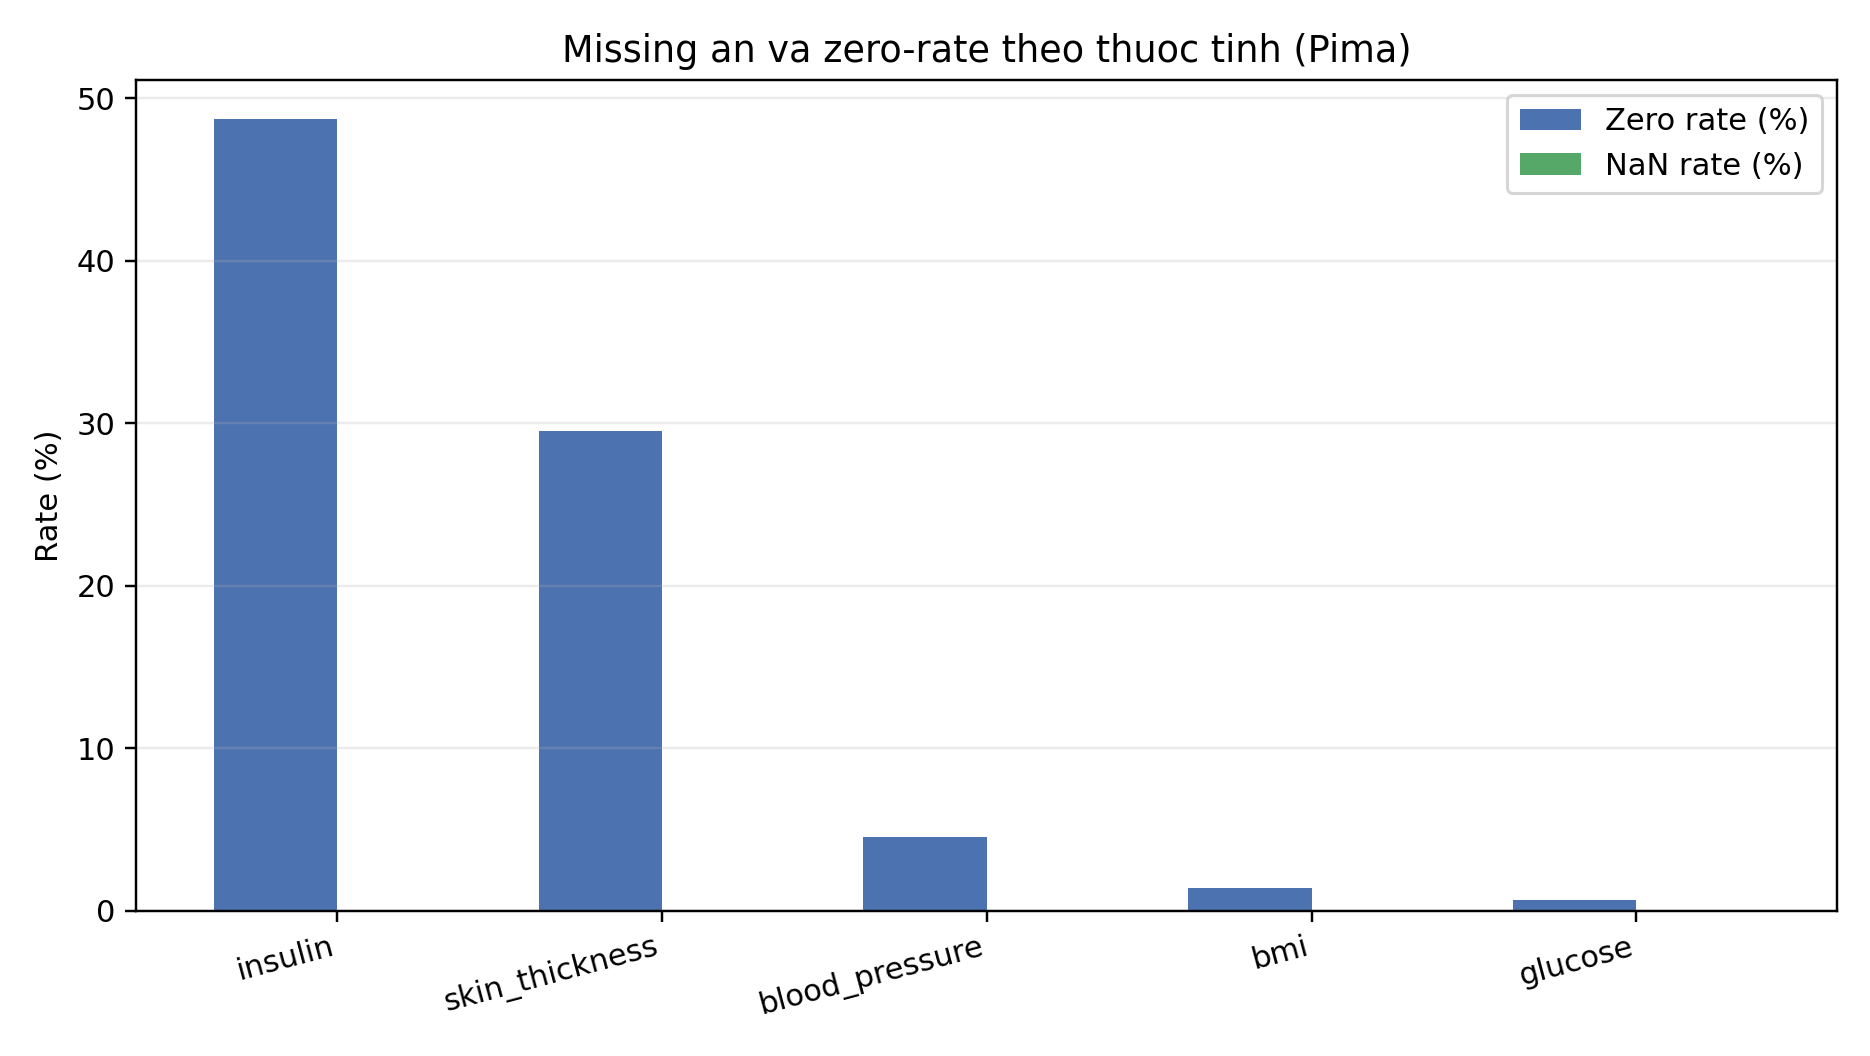
\includegraphics[width=0.82\linewidth]{figures/fig_missing_zero_report.png}
\caption{Thống kê missing ẩn và giá trị 0 theo thuộc tính}
\label{fig:missing_zero_report}
\end{figure}

\section{Quy trình tiền xử lý đề xuất}
Quy trình được đề xuất và triển khai trong notebook:
\begin{enumerate}[leftmargin=1.8em]
    \item Chuyển \texttt{0 -> NaN} cho các biến sinh lý bất thường.
    \item Chia dữ liệu theo tỉ lệ train/validation/test = 60/20/20 (stratified).
    \item Tạo pipeline kết hợp \textit{imputer + scaler + model}.
    \item So sánh 12 tổ hợp cấu hình (3 imputer x 2 scaler x 2 model).
\end{enumerate}

\begin{figure}[H]
\centering
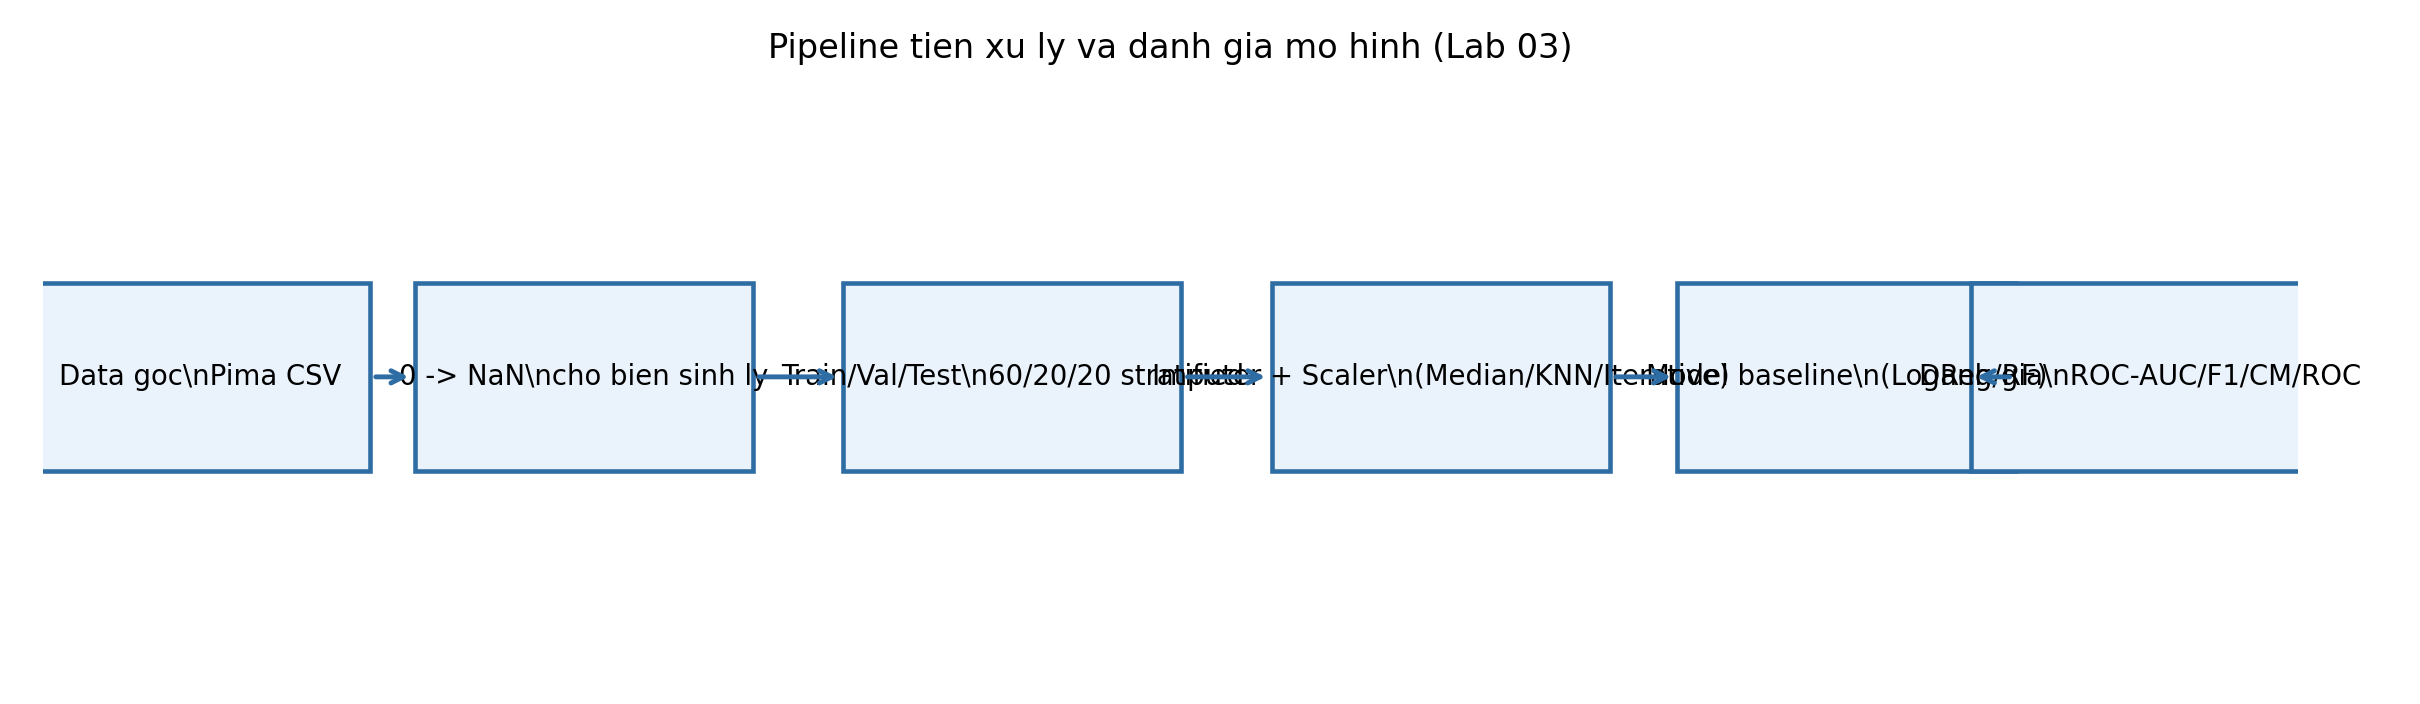
\includegraphics[width=0.62\linewidth]{figures/fig_preprocess_pipeline.png}
\caption{Pipeline tiền xử lý và đánh giá mô hình}
\label{fig:preprocess_pipeline}
\end{figure}

\chapter{Thuc nghiem va ket qua dat duoc}

\section{Thiet lap thuc nghiem}
\subsection{Chien luoc chia du lieu}
Du lieu duoc chia theo ti le 60/20/20 voi \textit{stratify} tren nhan \texttt{outcome}
de giu on dinh ti le lop duong tinh giua cac tap.
\begin{itemize}[leftmargin=1.5em]
    \item Train: 460 mau
    \item Validation: 154 mau
    \item Test: 154 mau
\end{itemize}

\subsection{To hop cau hinh duoc so sanh}
\begin{itemize}[leftmargin=1.5em]
    \item Imputation: Median, KNN, Iterative(MICE)
    \item Scaling: StandardScaler, MinMaxScaler
    \item Model: Logistic Regression, Random Forest
\end{itemize}
Tong cong 12 cau hinh duoc danh gia voi cung mot seed va cung mot split de dam bao cong bang.

\section{Ket qua EDA chinh}
\subsection{Tong quan bo du lieu}
Bo du lieu co 768 dong va 9 cot (8 bien dau vao va 1 bien dau ra).
Phan bo lop: class 0 = 500 mau (\~65.1\%), class 1 = 268 mau (\~34.9\%).

\begin{figure}[H]
\centering
\fbox{\parbox[c][5cm][c]{0.85\linewidth}{\centering
Placeholder Figure\\
Phan bo lop outcome}}
\caption{Phan bo lop trong du lieu Pima}
\label{fig:class_distribution}
\end{figure}

\subsection{Nhan xet ve quality data}
So dong trung lap bang 0. Cac cot co so luong \texttt{0} cao nhat la \texttt{insulin}
va \texttt{skin\_thickness}, do do can xu ly missing an truoc huan luyen.

\begin{figure}[H]
\centering
\fbox{\parbox[c][5cm][c]{0.85\linewidth}{\centering
Placeholder Figure\\
Heatmap tuong quan cac bien}}
\caption{Ma tran tuong quan sau khi ap dung zero-as-missing}
\label{fig:corr_heatmap}
\end{figure}

\section{So sanh mo hinh va chien luoc tien xu ly}
\subsection{Xep hang theo ROC-AUC}
Ket qua trong notebook cho thay cac cau hinh dan dau (theo test ROC-AUC) tap trung o
to hop KNN imputer + Random Forest.

\begin{table}[H]
\centering
\caption{Top cau hinh theo test ROC-AUC (trich tu notebook)}
\label{tab:top_configs}
\begin{tabular}{p{3cm}p{2.5cm}p{3cm}c}
\toprule
\textbf{Imputer} & \textbf{Scaler} & \textbf{Model} & \textbf{Test ROC-AUC}\\
\midrule
KNN & MinMax & Random Forest & 0.8170\\
KNN & Standard & Random Forest & 0.8168\\
Median & Standard & Logistic Regression & 0.8167\\
Iterative & MinMax & Random Forest & 0.8156\\
KNN & Standard & Logistic Regression & 0.8154\\
\bottomrule
\end{tabular}
\end{table}

\begin{figure}[H]
\centering
\fbox{\parbox[c][5cm][c]{0.85\linewidth}{\centering
Placeholder Figure\\
Barplot top strategies theo ROC-AUC va F1}}
\caption{So sanh cac cau hinh tien xu ly + mo hinh}
\label{fig:strategy_comparison}
\end{figure}

\subsection{Cau hinh de xuat}
Cau hinh tot nhat theo test ROC-AUC:
\textbf{KNN Imputer + MinMaxScaler + Random Forest}.
\begin{itemize}[leftmargin=1.5em]
    \item Validation ROC-AUC: 0.8700
    \item Test ROC-AUC: 0.8170
    \item Test F1: 0.6078
    \item Test Precision: 0.6458
    \item Test Recall: 0.5741
\end{itemize}

\section{Phan tich sai so va trade-off}
\subsection{Confusion matrix va ROC}
\begin{figure}[H]
\centering
\fbox{\parbox[c][5cm][c]{0.85\linewidth}{\centering
Placeholder Figure\\
Confusion matrix cho cau hinh tot nhat}}
\caption{Confusion matrix cua cau hinh duoc chon}
\label{fig:confusion_best}
\end{figure}

\begin{figure}[H]
\centering
\fbox{\parbox[c][5cm][c]{0.85\linewidth}{\centering
Placeholder Figure\\
ROC cua top 3 cau hinh}}
\caption{Duong cong ROC cho cac cau hinh dan dau}
\label{fig:roc_top3}
\end{figure}

\subsection{Trade-off theo threshold}
Notebook da thuc hien quet threshold va chi ra rang threshold 0.50 chua chac toi uu.
Diem can bang F1 tot nhat trong qua trinh quet nam quanh threshold xap xi 0.30,
cho thay neu uu tien phat hien ca duong tinh thi co the danh doi precision de tang recall.

\subsection{Nhan dinh overfitting/underfitting}
Chenh lech \texttt{val\_roc\_auc - test\_roc\_auc} xap xi 0.053.
Dieu nay cho thay dau hieu overfitting nhe den trung binh, can tiep tuc kiem chung bang
cross-validation va tuning he thong trong buoc tiep theo.

\chapter{Kết luận và khuyến nghị}

\section{Kết luận chung}
Báo cáo đã hoàn thành quy trình rút trích dữ liệu và tiền xử lý cho bài toán
dự đoán tiểu đường trên bộ dữ liệu Pima. Kết quả cho thấy việc kết hợp
\textit{zero-as-missing} với pipeline imputation + scaling là cần thiết để nâng cao
tính nhất quán của dữ liệu và hiệu năng mô hình baseline.

\section{Tóm tắt kết quả đạt được}
\begin{itemize}[leftmargin=1.5em]
    \item Hoàn thiện notebook phân tích theo hướng báo cáo học thuật.
    \item So sánh 12 cấu hình tiền xử lý và mô hình trên cùng điều kiện chia dữ liệu.
    \item Đề xuất cấu hình KNN + MinMax + Random Forest cho kết quả test ROC-AUC cao nhất.
    \item Bổ sung phân tích confusion matrix, ROC và threshold trade-off.
\end{itemize}

\section{Trả lời trực tiếp câu hỏi nghiên cứu (Q1/Q2/Q3)}
\begin{itemize}[leftmargin=1.5em]
    \item \textbf{Q1 -- Zero-as-missing có hữu ích không?}
    Có. Việc chuyển \texttt{0 -> NaN} cho các biến sinh lý giúp mô hình đạt mức AUC ổn định
    (test ROC-AUC quanh 0.81) thay vì để nhiễu từ giá trị 0 phi sinh lý.
    \item \textbf{Q2 -- Tổ hợp preprocessing/model nào tốt nhất?}
    Cấu hình tốt nhất là \textbf{KNN + MinMax + Random Forest} với
    \texttt{val\_roc\_auc=0.8700}, \texttt{test\_roc\_auc=0.8170}, \texttt{test\_accuracy=0.7403}.
    \item \textbf{Q3 -- Trade-off precision/recall thay đổi ra sao theo threshold?}
    Khi giảm ngưỡng từ 0.50 xuống 0.30, recall tăng mạnh từ 0.5741 lên 0.8148, trong khi precision
    giảm từ 0.6458 xuống 0.5789; F1 cải thiện từ 0.6078 lên 0.6769.
\end{itemize}

\section{Đóng góp của đề tài}
\begin{itemize}[leftmargin=1.5em]
    \item Chuẩn hóa quy trình thực hành từ EDA đến đánh giá mô hình baseline.
    \item Cung cấp khung đánh giá dễ tái lập cho các bài toán phân lớp y sinh tương tự.
    \item Tăng tính báo cáo hóa của notebook để phục vụ trình bày học phần.
\end{itemize}

\section{Hạn chế nghiên cứu}
\begin{enumerate}[leftmargin=1.8em]
    \item Quy mô dữ liệu còn nhỏ (768 mẫu), chưa đại diện cho nhiều quần thể bệnh nhân.
    \item Giả định \textit{zero-as-missing} có thể gây sai lệch nếu tồn tại trường hợp đo thực sự bằng 0.
    \item Đánh giá hiện tại dựa trên một lần chia train/validation/test, chưa có CV lặp lại.
    \item Chưa tiến hành tuning tham số hệ thống và calibration xác suất.
\end{enumerate}

\section{Hướng phát triển và kiến nghị}
\begin{enumerate}[leftmargin=1.8em]
    \item Áp dụng Stratified K-Fold CV để kiểm chứng độ ổn định kết quả.
    \item Mở rộng tuning tham số cho Logistic Regression và Random Forest.
    \item Thử nghiệm thêm các mô hình boosting (XGBoost/LightGBM) và kỹ thuật cân bằng lớp.
    \item Mở rộng bộ dữ liệu và kiểm tra external validity trên nguồn độc lập.
    \item Đóng gói pipeline suy luận và tạo báo cáo tự động để tăng khả năng triển khai.
\end{enumerate}


% References
\bibliographystyle{unsrtnat}
\bibliography{references}

\end{document}
